% !TEX root =  ../supplementary.tex
\section{A Bivariate Joint Model for the Longitudinal PSA, and DRE Measurements, and Time to Cancer Progression}
\label{sec:jm_framework}

In this appendix section, we first provide a short introduction to the world's largest active surveillance (AS) program called Prostate Cancer Research International Active Surveillance, abbreviated as PRIAS \citep{bokhorst2016decade}, that we use to develop our methodology. We then present an introduction to the joint models for time-to-event and longitudinal data \citep{tsiatis2004joint,rizopoulos2012joint}, that we fit to the PRIAS dataset. Lastly, we present the parameter estimation for our model using the Bayesian approach. 

\subsection{PRIAS Dataset}
The PRIAS dataset consists of 5270 AS patients, of which 866 observe cancer progression. For each patient, prostate-specific antigen (PSA) measurements (ng/mL) are scheduled every 3 months for first 2 years and every 6 months thereafter. The DRE measurements are scheduled every 6 months. We use the DRE measurements after converting them on a binary scale, namely ${\mbox{DRE} > \mbox{T1c}}$ and ${\mbox{DRE} \leq \mbox{T1c}}$ \citep{schroder1992tnm}. On average 5 DRE and 9 PSA measurements have been recorded per patient. Larger values for PSA and/or larger score for DRE, may indicate cancer progression. However, it is the occurrence of biopsy Gleason score larger than 6, that is commonly considered as cancer progression. In the PRIAS study, biopsies are scheduled at the  following fixed follow-up times (measured since inclusion in AS): year 1, 4, 7, and 10, and every 5 years thereafter. An annual schedule of biopsies is prescribed to those patients who have a PSA doubling time between 0 and 10 years. The PSA doubling time at any point during follow-up is measured as the inverse of the slope of the regression line through the base two logarithm of the observed PSA values.

In Figure~\ref{fig:npmle_plot}, we show the survival probability of cancer progression estimated using the cancer progression times observed for the patients from the PRIAS program. Prostate cancer is a slowly progressing disease, which is evident by the 50\% probability of not having a cancer progression by the end of the ten year follow-up period.

\begin{figure}[!htb]
\captionsetup{justification=justified}
\centerline{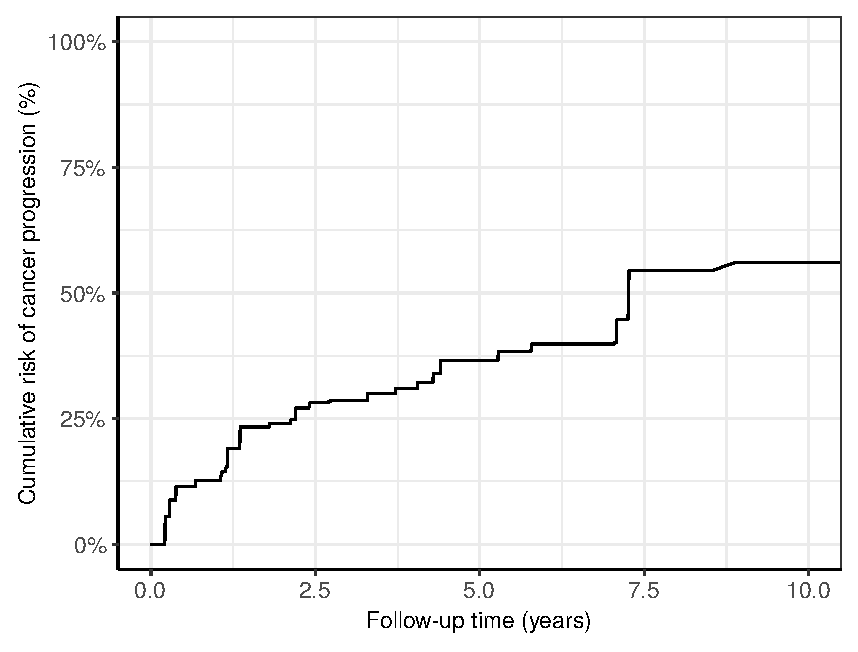
\includegraphics[width=\columnwidth]{images/npmle_plot.eps}}
\caption{\textbf{Estimated survival probability of cancer progression in AS}: for patients in the Prostate Cancer Research International Active Surveillance (PRIAS) dataset. Roughly 50\% patients (\textit{slow progressing}) do not progress in the ten year follow-up period. Estimation is done using a nonparametric maximum likelihood estimate, of the distribution function for interval censored cancer progression times \citep{turnbull1976empirical}.}
\label{fig:npmle_plot}
\end{figure}

\subsection{Model Definition}
\label{subsec:model_def}
Let $T_i^*$ denote the true cancer progression time of the $i$-th patient included in PRIAS. Since biopsies are conducted periodically, $T_i^*$ is observed with interval censoring ${l_i < T_i^* \leq r_i}$. When progression is observed for the patient at his latest biopsy time $r_i$, then $l_i$ denotes the time of the second latest biopsy. Otherwise, $l_i$ denotes the time of the latest biopsy and $r_i = \infty$. Further, let $\boldsymbol{y}_{di}$, and $\boldsymbol{y}_{pi}$ denote the $n_{di} \times 1$, and $n_{pi} \times 1$ vectors of the DRE, and PSA longitudinal measurements, respectively. The observed data of all $n$ patients is denoted by ${\mathcal{D}_n = \{l_i, r_i, \boldsymbol{y}_{di}, \boldsymbol{y}_{pi}; i = 1, \ldots, n\}}$.

\begin{figure}[!htb]
\captionsetup{justification=justified}
\centerline{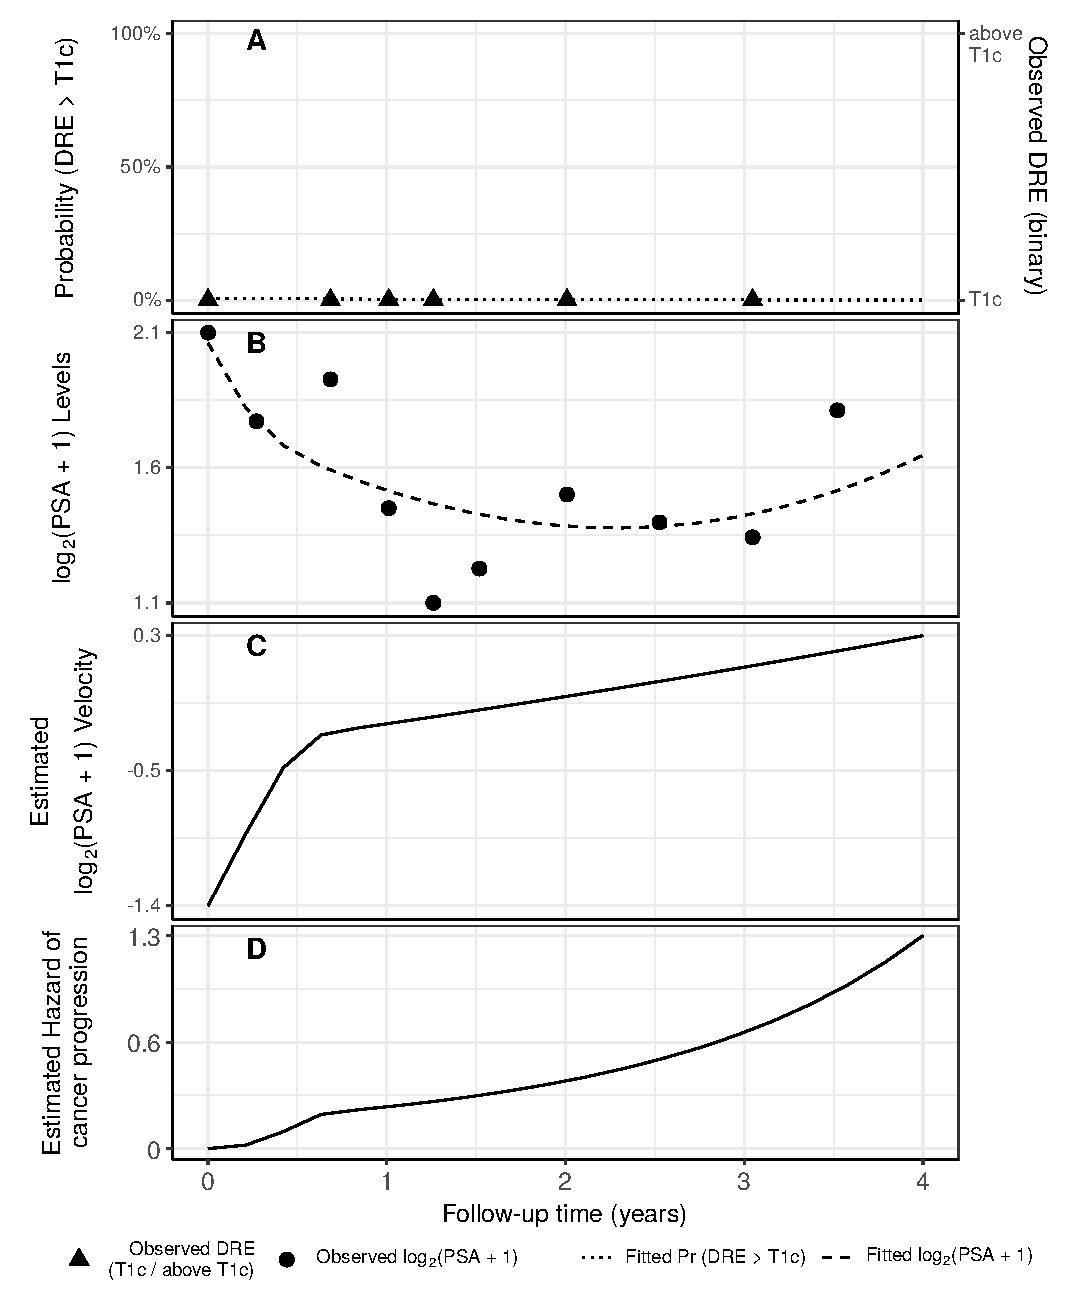
\includegraphics[width=\columnwidth]{images/jmExplanationPlot_1757.eps}}
\caption{\textbf{Illustration of the joint model fitted to the PRIAS dataset}. \textbf{Panel~A:} shows the observed DRE scores and the fitted probability of obtaining a DRE score greater than T1c (Equation~\ref{eq:long_model_dre}) for . \textbf{Panel~B:} shows the observed and fitted $\log_2(\mbox{PSA} + 1)$ levels (Equation~\ref{eq:long_model_psa}). \textbf{Panel~C:} shows the estimated $\log_2(\mbox{PSA} + 1)$ velocity (velocity cannot be observed directly) over time. The hazard function (Equation~\ref{eq:rel_risk_model}) shown in \textbf{Panel~D}, depends on the fitted log odds of having a $\mbox{DRE} > \mbox{T1c}$, and the fitted $\log_2(\mbox{PSA} + 1)$ value and velocity.}
\label{fig:jmExplanationPlot_1757}
\end{figure}

In our joint model, the patient-specific PSA and DRE measurements over time are modeled using a bivariate generalized linear mixed effects sub-model. The sub-model for DRE is given by (see Panel~A, Figure~\ref{fig:jmExplanationPlot_1757}):
\begin{equation}
\label{eq:long_model_dre}
\begin{split}
    \mbox{logit} \big[\mbox{Pr}\{y_{di}(t) > \mbox{T1c}\}\big] &= \beta_{0d} + b_{0di} + (\beta_{1d} + b_{1di}) t\\
    &+ \beta_{2d} (\mbox{Age}_i-70) + \beta_{3d} (\mbox{Age}_i-70)^2
    \end{split}
\end{equation}
where, $t$ denotes the follow-up visit time, and $\mbox{Age}_i$ is the age of the ${i\mbox{-th}}$ patient at the time of inclusion in AS. The fixed effect parameters are denoted by ${\{\beta_{0d}, \ldots, \beta_{3d}\}}$, and ${\{b_{0di}, b_{1di}\}}$ are the patient specific random effects. With this definition, we assume that the patient-specific log odds of obtaining a DRE score larger than T1c remain linear over time. 

The mixed effects sub-model for PSA is given by (see Panel~B, Figure~\ref{fig:jmExplanationPlot_1757}):
\begin{equation}
\label{eq:long_model_psa}
\begin{split}
    \log_2 \big\{y_{pi}(t) + 1\big\} &= m_{pi}(t) + \varepsilon_{pi}(t),\\
    m_{pi}(t) &= \beta_{0p} + b_{0pi} + \sum_{k=1}^4 (\beta_{kp} + b_{kpi})  B_k(t,\mathcal{K})\\ 
    &+ \beta_{5p} (\mbox{Age}_i-70) + \beta_{6p} (\mbox{Age}_i-70)^2,
    \end{split}
\end{equation}
where, $m_{pi}(t)$ denotes the underlying measurement error free value of $\log_2 (\mbox{PSA} + 1)$ transformed \citep{pearson1994mixed,lin2000latent} measurements at time $t$. We model it non-linearly over time using B-splines \citep{de1978practical}. To this end, our B-spline basis function $B_k(t, \mathcal{K})$ has 3 internal knots at $\mathcal{K} = \{0.1, 0.7, 4\}$ years, and boundary knots at 0 and 5.42 years (95-th percentile of the observed follow-up times). The fixed effect parameters are denoted by ${\{\beta_{0p},\ldots,\beta_{6p}\}}$ and ${\{b_{0pi}, \ldots, b_{4pi}\}}$ are the patient specific random effects. The error $\varepsilon_{pi}(t)$ is assumed to be t-distributed with three degrees of freedom (see \ref{subsec:t-dist-assumption}) and scale $\sigma$, and is independent of the random effects. 

To account for the correlation between the DRE and PSA measurements of a patient, we link their corresponding random effects. More specifically, the complete vector of random effects ${\boldsymbol{b}_i = (b_{0di}, b_{1di}, b_{0pi}, \ldots, b_{4pi})^T}$ is assumed to follow a multivariate normal distribution with mean zero and variance-covariance matrix $\boldsymbol{D}$.

To model the impact of DRE and PSA measurements on the risk of cancer progression, our joint model uses a relative risk sub-model. More specifically, the hazard of cancer progression $h_i(t)$ at a time $t$ is given by (see Panel~D, Figure~\ref{fig:jmExplanationPlot_1757}):
\begin{equation}
\label{eq:rel_risk_model}
\begin{split}
    h_i(t) &= h_0(t) \exp\Big(\gamma_1 (\mbox{Age}_i-70) + \gamma_2 (\mbox{Age}_i-70)^2\\
    &+\alpha_{1d} \mbox{logit} \big[\mbox{Pr}\{y_{di}(t) > \mbox{T1c}\}\big]+ \alpha_{1p} m_{pi}(t) + \alpha_{2p} \frac{\partial m_{pi}(t)}{\partial {t}}\Big),
    \end{split}
\end{equation}
where, $\gamma_1, \gamma_2$ are the parameters for the effect of age. The parameter $\alpha_{1d}$ models the impact of log odds of obtaining $\mbox{DRE} > \mbox{T1c}$ on the hazard of cancer progression. The impact of PSA on the hazard of cancer progression is modeled in two ways: a) the impact of the error free underlying PSA value $m_{pi}(t)$ (see Panel~B, Figure~\ref{fig:jmExplanationPlot_1757}), and b) the impact of the underlying PSA velocity $\partial m_{pi}(t)/\partial {t}$ (see Panel~C, Figure~\ref{fig:jmExplanationPlot_1757}). The corresponding parameters are $\alpha_{1p}$ and $\alpha_{2p}$, respectively. Lastly, $h_0(t)$ is the baseline hazard at time t, and is modeled flexibly using P-splines \citep{eilers1996flexible}. More specifically:
\begin{equation*}
\log{h_0(t)} = \gamma_{h_0,0} + \sum_{q=1}^Q \gamma_{h_0,q} B_q(t, \boldsymbol{v}),
\end{equation*}
where $B_q(t, \boldsymbol{v})$ denotes the $q$-th basis function of a B-spline with knots $\boldsymbol{v} = v_1, \ldots, v_Q$ and vector of spline coefficients $\gamma_{h_0}$. To avoid choosing the number and position of knots in the spline, a relatively high number of knots (e.g., 15 to 20) are chosen and the corresponding B-spline regression coefficients $\gamma_{h_0}$ are penalized using a differences penalty \citep{eilers1996flexible}. An example fitted hazard is shown in panel D of Figure~\ref{fig:jmExplanationPlot_1757}.  

\subsection{Parameter Estimation}
We estimate the parameters of the joint model using Markov chain Monte Carlo (MCMC) methods under the Bayesian framework. Let $\boldsymbol{\theta}$ denote the vector of all of the parameters of the joint model. The joint model postulates that given the random effects, the time to cancer progression, and the PSA and DRE measurements taken over time are all mutually independent. Under this assumption the posterior distribution of the parameters is given by:
\begin{align*}
p(\boldsymbol{\theta}, \boldsymbol{b} \mid \mathcal{D}_n) & \propto \prod_{i=1}^n p(l_i, r_i, \boldsymbol{y}_{di}, \boldsymbol{y}_{pi}, \mid \boldsymbol{b}_i, \boldsymbol{\theta}) p(\boldsymbol{b}_i \mid \boldsymbol{\theta}) p(\boldsymbol{\theta})\\
& \propto \prod_{i=1}^n p(l_i, r_i \mid \boldsymbol{b}_i, \boldsymbol{\theta}) p(\boldsymbol{y}_{di} \mid \boldsymbol{b}_i, \boldsymbol{\theta}) p(\boldsymbol{y}_{pi} \mid \boldsymbol{b}_i, \boldsymbol{\theta}) p(\boldsymbol{b}_i \mid \boldsymbol{\theta}) p(\boldsymbol{\theta}),\\
p(\boldsymbol{b}_i \mid \boldsymbol{\theta}) &= \frac{1}{\sqrt{(2 \pi)^q \text{det}(\boldsymbol{D})}} \exp(\boldsymbol{b}_i^T \boldsymbol{D}^{-1} \boldsymbol{b}_i),
\end{align*}
where, the likelihood contribution of the DRE outcome, conditional on the random effects is:
\begin{equation*}
p(\boldsymbol{y}_{di} \mid \boldsymbol{b}_i, \boldsymbol{\theta}) = \prod_{k=1}^{n_{di}} \frac{\exp\Big[-\mbox{logit} \big\{\mbox{Pr}(y_{dik} > \mbox{T1c})\big\} I(y_{dik}=\mbox{T1c}) \Big]}  {1+\exp\Big[-\mbox{logit} \big\{\mbox{Pr}(y_{dik} > \mbox{T1c})\big\}\Big]},
\end{equation*}
where $I(\cdot)$ is an indicator function which takes the value 1 if the $k$-th repeated DRE score ${y_{dik}=\mbox{T1c}}$, and takes the value 0 otherwise. The likelihood contribution of the PSA outcome, conditional on the random effects is:
\begin{equation*}
p(\boldsymbol{y}_{pi} \mid \boldsymbol{b}_i, \boldsymbol{\theta}) = \frac{1}{\big(\sqrt{2 \pi \sigma^2}\big)^{n_{pi}}} \exp\bigg(-\frac{{\lVert{\boldsymbol{y}_{pi} - \boldsymbol{m}_{pi}}\rVert}^2}{\sigma^2}\bigg),
\end{equation*}
The likelihood contribution of the time to cancer progression outcome is given by:
\begin{equation}
\label{web_eq : likelihood_contribution_survival}
p(l_i,r_i\mid \boldsymbol{b}_i,\boldsymbol{\theta}) = \exp\Big\{-\int_0^{l_i} h_i(s)\mathrm{d}{s}\Big\} - \exp\Big\{-\int_0^{r_i}h_i(s)\mathrm{d}{s}\Big\}.
\end{equation}
The integral in (\ref{web_eq : likelihood_contribution_survival}) does not have a closed-form solution, and therefore we use a 15-point Gauss-Kronrod quadrature rule to approximate it.

We use independent normal priors with zero mean and variance 100 for the fixed effects ${\{\beta_{0d},\ldots,\beta_{3d}, \beta_{0p},\ldots,\beta_{6p}\}}$, and inverse Gamma prior with shape and rate both equal to 0.01 for the parameter $\sigma^2$. For the variance-covariance matrix $\boldsymbol{D}$ of the random effects we take inverse Wishart prior with an identity scale matrix and degrees of freedom equal to 7 (number of random effects). For the relative risk model's parameters $\{\gamma_1, \gamma_2\}$ and the association parameters $\{\alpha_{1d}, \alpha_{1p}, \alpha_{2p}\}$, we use independent normal priors with zero mean and variance 100.

\subsection{Personalized Posterior Predictive Distribution of Time of Cancer Progression}
Let us assume a new patient $j$, for whom we need to make a personalized biopsy decision. Let his current follow-up visit time be $s$, latest time of biopsy be $t\leq s$, observed vectors of DRE and PSA measurements be $\mathcal{Y}_{dj}(s)$ and $\mathcal{Y}_{pj}(s)$, respectively. The combined information from the observed data is given by the following posterior predictive distribution $g(T^*_j)$ of his time of cancer progression $T^*_j$:
\begin{equation*}
\label{eq:post_pred_dist}
\begin{aligned}
g(T^*_j) &= p\big\{T^*_j \mid T^*_j > t, \mathcal{Y}_{dj}(s), \mathcal{Y}_{pj}(s), \mathcal{D}_n\big\}\\
&= \int \int p\big(T^*_j \mid T^*_j > t, \boldsymbol{b}_j, \boldsymbol{\theta}\big)\\
&\times p\big\{\boldsymbol{b}_j \mid T^*_j>t, \mathcal{Y}_{dj}(s), \mathcal{Y}_{pj}(s), \boldsymbol{\theta}\big\}p\big(\boldsymbol{\theta} \mid \mathcal{D}_n\big) \mathrm{d} \boldsymbol{b}_j \mathrm{d} \boldsymbol{\theta}.
\end{aligned}
\end{equation*}
The distribution $g(T^*_j)$ depends on observed data of the patient $\mathcal{Y}_{dj}(s)$ and $\mathcal{Y}_{pj}(s)$, as well information from the PRIAS dataset $\mathcal{D}_n$ via the posterior distribution of random effects $\boldsymbol{b}_j$ and posterior distribution of the vector of all parameters $\boldsymbol{\theta}$, respectively.

The distribution can be estimated as detailed in \citet{landmarking2017}. However, majority of the prostate cancer patients do not progress in the ten year follow-up period of PRIAS (see Figure~\ref{fig:npmle_plot}). Consequently, the personalized density function of cancer progression $g(T^*_j)$ can only be estimated for time points falling within the ten year follow-up. 